\documentclass[../Proposal.tex]{subfiles}

\begin{document}
% Describe the general data patterns, as emerging from your measurements. Depict these patterns in terms of graphs, charts, and/or tables. 
% Compute your descriptive statistics (means and standard deviations). See what these descriptive stats tell you about the hypotheses you put forth earlier. 
While preprocessing, some items were excluded, either because some gestures could not be labelled or because the timing relations between the gestures deviated too much from the others. This left \input{numbers/instances.txt} instances of measured words.\\
First of all, a \input{numbers/ttest_length_method.txt} revealed that indeed, stressed syllables are significantly  ($p<0.001$: p = \input{numbers/ttest_length_pvalue.txt}) longer in duration than unstressed syllables when comparing the intervals between the left edge and the anchor. Violin plots of the distribution of syllable lengths depending on stress are illustrated in \cref{fig:syll_length}. The estimated mean duration value for stressed syllables is \input{numbers/ttest_length_estx.txt}ms and for unstressed syllables \input{numbers/ttest_length_esty.txt}ms.
We can therefore confirm what was already stated in \cref{sec:lit} after \cite{prieto2018prosody} that stressed syllables are longer than unstressed syllables and see that stress in general has an influence on syllables. 
In the following we will see the influence of stress on the general temporal organization of a syllable.\\

\begin{figure}
    \centering
    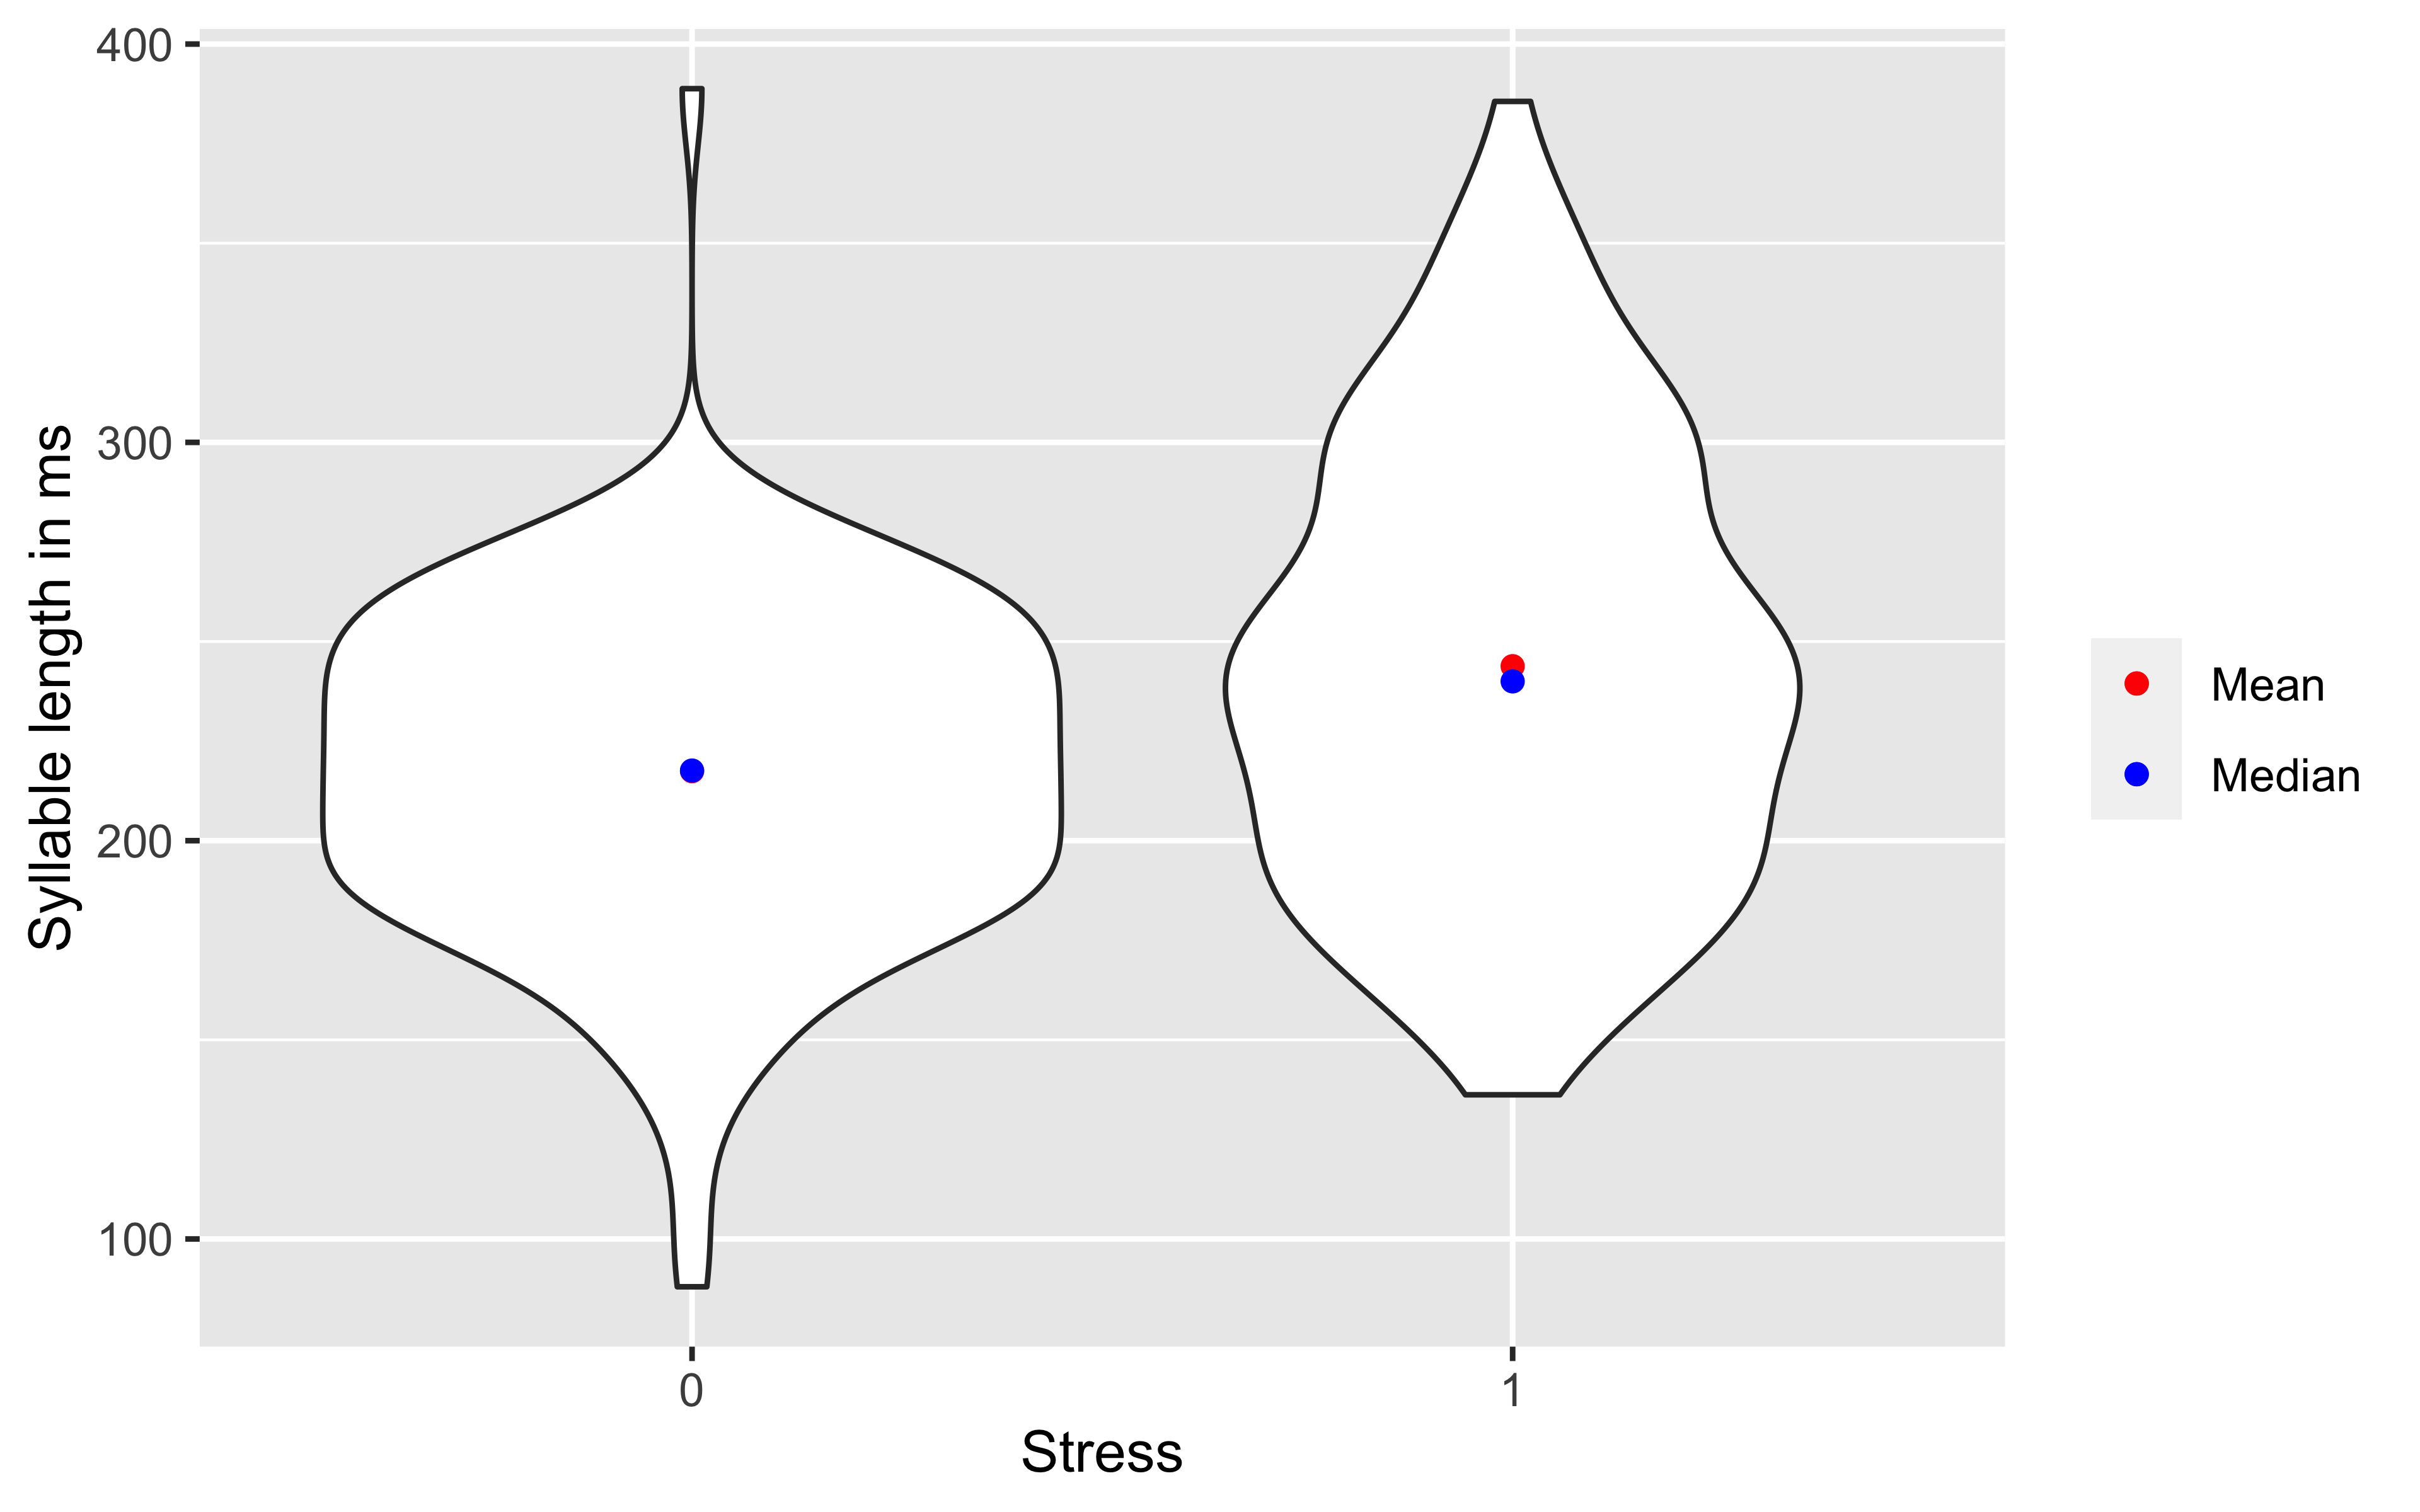
\includegraphics[width=12cm]{figures/syll_length.png}
    \caption{Violin plot of syllable length depending on stress.}
    \label{fig:syll_length}
\end{figure}
 
%%%%%%%%
\cref{tab:rel_sds} shows the RSDs of the three intervals for all items, split by stress or no stress. In both cases, the c-center to anchor interval is almost always the least variable, ergo one could speak of c-center stability. However, if we look at the values broken down into \cref{tab:all_pairs}, we can see exceptions to this. Interestingly, the finding of \cite[]{sotiropoulou2020global} that voiced stop-lateral clusters exhibit local timing interval stability can be reproduced, but only for stressed syllables and additionally for stressed voiceless syllables, whose nucleus is /e/. Unstressed syllables show overall global timing interval stability.
\\
However, it must also be noted that the differences between the RSD values are sometimes very small. In any case, we can observe that there is a difference between stressed and unstressed syllables, because stressed syllables generally seem to have greater variability in their interval lengths. 
% latex table generated in R 4.0.2 by xtable 1.8-4 package
% Wed Nov  9 18:00:06 2022
\begin{table}[ht]
\centering
\begin{tabular}{rlrrr}
  \hline
 & Stressed\_syllable & LE & CC & RE \\ 
  \hline
1 & yes & 22.61 & 21.28 & 22.22 \\ 
  2 & no & 19.24 & 18.86 & 21.71 \\ 
   \hline
\end{tabular}
\caption{Relative standard deviations  of interval length between left edge (LE), C-Center (CC) and right edge (RE) and the anchor, respectively.\label{tab:rel_sds}} 
\end{table}

% latex table generated in R 4.0.2 by xtable 1.8-4 package
% Wed Nov  9 18:00:20 2022
\begin{table}[ht]
\centering
\begin{tabular}{rlrrrrrrrr}
  \hline
 & Landmark & blA & blE & plA & plE & bla & ble & pla & ple \\ 
  \hline
1 & LE & 19.66 & 26.04 & 18.64 & 26.64 & 18.76 & 17.97 & 22.13 & 19.82 \\ 
  2 & CC & 17.70 & 23.96 & 17.76 & 22.94 & 17.91 & 17.64 & 21.48 & 17.69 \\ 
  3 & RE & 17.40 & 22.58 & 21.69 & 21.18 & 18.80 & 20.70 & 23.55 & 20.30 \\ 
   \hline
\end{tabular}
\caption{Relative standard deviations of interval length between left edge (LE), C-Center (CC) and right edge (RE) and the anchor, respectively. Broken down by syllable type; capitalization of letters indicates stress.\label{tab:all_pairs}} 
\end{table}

\\
It could be that there is an interaction of stress and vowel, as stressed syllables with /e/ in the nucleus have the largest RSDs and unstressed voiced syllables with /a/ in the nucleus have the smallest variables, thus are show the most stable timing relations.\\

%% Discussion
%Discuss your findings and their significance, i.e. what do your findings mean about the phenomenon you set out to study in this paper. Discuss possible confounds and problems with the data. Point out any relation (agreement, contradiction, extension etc.) between your findings and those made by other authors whose work you may have read in this class or elsewhere.
The fact that variability in stressed syllables is slightly higher, is surprising since I hypothesized that longer syllable durations will be compensated through normalizing with the mean when calculating the RSD and no particular differences between stressed and unstressed syllables will be found. 
This higher variability in the temporal organization could be because stressed syllables are more marked than their unstressed counterparts. A hypothetical explanation could be that unstressed syllables are more prototypical and `unstressing' mitigates the influences of parameters such as voicing on the relations between gestures.\\
Nonetheless it has to be noted that I did not compute whether the differences between stressed and unstressed syllables are statistically significant, doing that would have been out of scope of this paper. 
In comparison to other papers, the calculated RSDs are relatively large. Whether this is because of the fact, that the dataset is comparatively small (only two speakers, two different vowels, only stop-lateral clusters) or because word medial clusters are different to word initial clusters, is not clear. Labelling and analyzing the rest of the corpus will surely shine some light into that.

\end{document}